\documentclass{extarticle}

\usepackage{graphicx}
\usepackage{enumerate}
\usepackage{amsthm}
\usepackage{amsmath}
\usepackage[titletoc,title]{appendix}
\usepackage[margin=1.0in]{geometry}
\usepackage[hypcap]{caption}
\DeclareGraphicsExtensions{.pdf,.png,.jpg}

% Needs to be last. Blue links look better to me than red boxes and red links
\usepackage[colorlinks=true,linkcolor=blue]{hyperref}

\begin{document}

\begin{titlepage}
\title{Design Document for Kairos Constraint-Based Scheduling Software System}
\author{Tyler Chapman, Nate Crandall, Vinh Dang, Vince Oveson, Tony Tuttle}
% INSERT TEAM LOGO
\maketitle
\thispagestyle{empty}
\end{titlepage}

\tableofcontents
\listoffigures

\newpage

\section{Executive Summary} % ONE PAGE

\subsection{Overview}
% DESCRIBE THE FINAL GOAL OF THE PROJECT
%   - what the project will do
The final goal of the project is to provide a highly customizable, open-source, web-based scheduling tool available
to solve a wide range of scheduling problems.  Our software system will be accessible through a public
website where users may build, modify, and maintain their solutions.  The system will be capable of solving various
types of scheduling problems for various types of user needs.

%   - what need it will address
Scheduling problems are ubiquitous.  Individuals, teams, organizations, and larger entities such as companies all
must solve scheduling problems of various levels of complexity.  Our tool aims to address the needs of such a wide
base of potential users.

\subsection{Features and Components}
% LIST KEY FEATURES AND COMPONENTS
%   - schedule solver
%   - web-based (open to all users)
%   - customizable
%   - well-written API
%   - thoughtful visualization component
At its core, Kairos will be a web-based schedule solver; it will accept parameters from the user, specifying the
details of their particular scheduling problem.  The tool will analyze the input and algorithmically determine a
schedule that will meet all of the supplied parameters.  If meeting all of the constraints is not possible, it will
prioritize based on weights and determine what compromises to make in the schedule.

Since the tool will be web-based, it will be open to any and all potential users.  This will further encourage a
wide breadth of users.

We intend to make the tool extremely customizable by creating a very general schedule solver core.
We want users to have access to the powerful core components while maintaining sufficient flexibility to fit the
solution to their specific needs.

Part of this customizability will come from working hard to make the API as clear and thorough as possible.  A
great piece of software may lose potential users if it is not clear to users how best to leverage the software.  We
intend to encourage a large user base by putting a lot of emphasis on creating a strong API.

Likewise, a great piece of software that lacks intuitiveness or a pleasing user experience will alienate users.
We will put a great deal of thought and planning into determining how best to use visualization tools to represent
our data.  Since scheduling is a complex problem that produces data that will need to be viewed from several angles,
this is a difficult problem in itself.  By making visualization a priority we hope to attract users as opposed to
driving them away.

\subsection{Justification}
% EXPLAIN WHY THE PROJECT IS INTERESTING AND WORTHWHILE
%   - why a completed project will be beneficial
Making this tool available to the public will potentially save individuals a great deal of time, provide
organizations better scheduling solutions than they currently have, and save a great deal
of money for businesses and other organizations.  At the very least, it is our hope that we will make life a little
easier for as many users as possible.

\section{Background}

\subsection{Overview} % ONE TO THREE PAGES
%   - why our project is needed
The task of creating optimal schedules is a problem that event planners, groups, teams, and other organizations of
all sizes encounter on a regular basis.  The schedules used by these groups are often created manually.  For all
but the simplest schedules, this task is extremely complicated and time consuming.  As the complexity increases,
the difficulty of creating acceptable schedules, much less optimal ones, increases exponentially.

%   - what problems it solves
Moving as much of the work of scheduling from a manual process to one that is solved by a computer is the
inspiration for Kairos.  Kairos has the potential to save a great deal of time for users.  Kairos will provide a
better solution for those who need to schedule any but the simplest of events.

%   - who will use it
Since scheduling is a ubiquitous problem, Kairos will be usable to large number of users.  By implementing a
well-documented API we intend to attract those who seek a solution that they can tweak to fit their specific needs.

A specific use case that we have identified is the School of Computing at the University of Utah.  We are working
with staff in the department to provide a solution to their problem of scheduling classes each semester.

\subsubsection{Similar Ideas}
% list, describe other software systems that do what ours will do
We have identified two software systems that address the scheduling problem in some manner similar to that which
we are aiming at.  These systems are Aurora Intelligent Planning and Scheduling System (Aurora) and Microsoft
Project (MS Project).  To be sure, there are other software systems out there, but these are adequate to represent
the current state of this space.

\subsubsection{How Kairos is Different}
% explain why our idea is different and/or better
Based on their literature, Aurora addresses the needs that we are attempting to address more than adequately.
However, they are focused on supplying solutions to very large organizations with correspondingly very large
scheduling problems.  We would like to address the needs of the smaller users for which the Aurora software would
be overkill.

While MS Project does include scheduling tools in the software package, the larger goal of MS Project is to provide
project management software.  Thus, their software is attempting to address a problem with a wider scope than we
are focused on.  Based on reading the literature on their software, it is not clear that the scheduling tools
provided in MS Project are constraint-based scheduling tools.

Both Aurora and MS Project cost money.  Our software will be free.  Neither Aurora or MS Project are web-based, but
require installation on any machine that will use the software.  There is certainly room for our tool in this
space.

\subsection{Required Technology}
% list, describe software technologies that you will:
%   - need to implement
%   - need to utilize
Our project can be broken down into three main components:  a core web service, specific modules that connect to
it, and an API that handles communication between the two.  We will discuss the technologies we plan to utilize in
developing each of these three components.

\subsubsection{Core Web Service}
This is where the logic for the schedule solver will live.  This web service will be centered around the transfer
of data through requests and responses.  Our web service will use API keys to restrict access.  In order to
authenticate users, we will store these keys in a MySQL database.  This will make our web service more secure.

\subsubsection{SoC Module}
We will create a module for the School of Computing that connects to our web service.  This module will be a web
application that allows the user to specify the events (classes) to be scheduled, the resources to be used
(professors, rooms, etc.), and the constraints for both classes and resources.  When the web service sends back a
suggested schedule, the user will be provided with different options for viewing the data.  We also plan to provide
some web scraping tools in order to facilitate the collection of data relevant to scheduling classes.

This module with have a PHP backend, along with a MySQL database.  The front end will be built using HTML,
JavaScript, and CSS.  We will utilize jQuery (specifcally ajax) to make asynchronous requests to the web
service without interrupting the user experience.

\subsubsection{API}
Our API will use JSON to represent the data being shuttled back and forth between the web service and the modules
which connect to it.  We plan to provide detailed documentation that will help other developers leverage our
service in their own applications.  To make this documentation readily available and accessible, we will create a
website where we will publish the API documentation, and also advertise our service.  This site will also be where
developers can request an API key.

\subsection{Assets and Engines}
% assets and engines
%   - how much will be built from scratch
%   - what resources, assets (and from where) will be leveraged
The websites we create -- both the API documentation site and the School of Computing module -- will be built using
the Laravel Artisan PHP framework.  This will provide structure to our web sites, as well as allow us to keep our
code organized and concise.  Laravel also includes a command line interface which will provide us with shortcuts
for common tasks, thus allowing us to focus our efforts on more important development tasks.

\subsection{Software/Hardware Requirements for Users}
% what hardware, software we will need to successfully installed in order to use our software
Since Kairos will be a web application with all of the intensive computation taking place on our network, the only
system requirements for users will be a machine running a modern browser with a reasonably fast internet connection.

\section{Requirements Analysis}

\subsection{System Architecture}
% how we envision the system from the developer's point of view
% what components will be necessary to meet the use cases
% could benefit from figure(s)
% ~ if figures take up too much space, put them in an appendix
% this section should address all the components/modules of your system and how they will communicate

\subsubsection{Constraint Solver}
At the core of our system will be the constraint solver.  The constraint solver is the software that solves general
constraint-based scheduling problems.  The solver will receive the parameters of a problem instance from the app
server and will return a solution back to the app server if one is discovered.  The solver will be written in Java
and will make use of one or more constraint programming libraries.

A problem instance will be supplied to the solver as a set of activities, a set of resources, a set of constraints,
and some objective function.  The solver will attempt to fulfill the objective function given the resources and
constraints and, if successful, will return a solution to the app server.  If it is not possible to fulfill the
objective function, a message indicating such will be returned.

\subsubsection{App Server}
The app server will be the means by which the constraint solver communicates with its users.  These users will be
one of two types.  The first type is the API user.  API users will use the solver to solve general scheduling
problems.  They are converting their concrete scheduling problems into instances of general constraint problems and
providing those problem details to the solver.  When they receive a solution they will convert it back in order to
apply it to their specific scheduling problem.

The second potential user of the app server will be our own Apache server.  Similarly to the API user, the problem
will be supplied from the Apache server as a general constraint problem.  The difference is that these problems will
be generated from our implementation of the class scheduler for University of Utah classes.

\subsubsection{Apache Server}
The Apache server will serve our API documentation website as well as the University of Utah class scheduler site,
and the School of Computing class scheduler tool.  The API documentation site will be the reference for our API
users.  It will include all of documentation necessary in order for API users to leverage our solver.  It will
provide detailed explanations of the methods available as well as code examples.

The University of Utah class scheduler site will presently be a site that will be set up such that departments at
the University will be easily able to begin using our scheduling tool.  Additionally, it will be extended to fit the
specific needs of our primary test user, the School of Computing.

\begin{figure}[!ht]
\centering
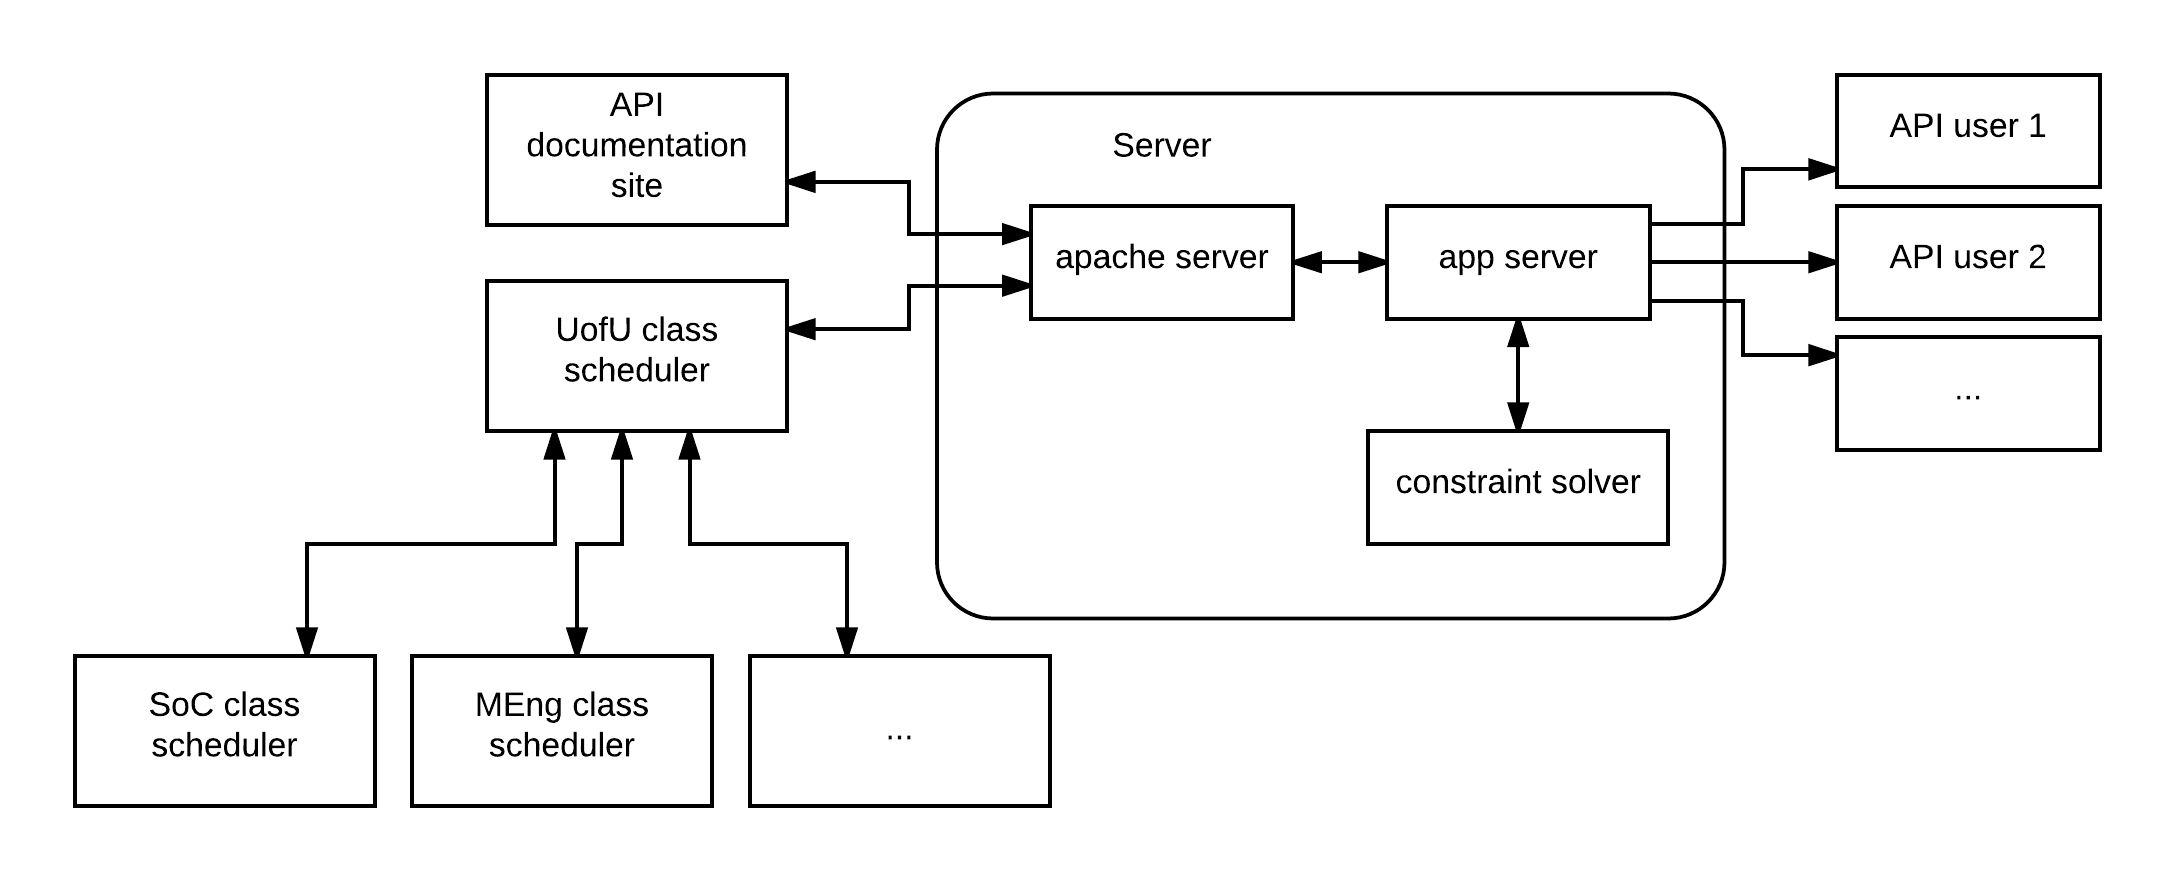
\includegraphics[width=1.0\textwidth]{img/general_sys_arch}
\caption{Overview of the System}
\label{fig:sys_arch}
\end{figure}

\subsection{Personnel}
% main responsibilities of each team member
% every team member must contribute substantially

We have five team members that will work together to implement this project in its entirety.  The members are
Tyler Chapman, Nate Crandall, Vinh Dang, Vince Oveson, and Tony Tuttle.

Tyler's primary responsibilities will be ensuring that the network functions correctly and securely.  As an
extension to his responsibilities to manage the network, Tyler will be the primary person responsible for
implementing the server back-end.

Nate's primary responsibility will be to develop the visualization component of the project.  He will be working
closely with the front-end developer and will use his knowledge of visualization to make sure that our the user
interface will maximize usability and aethetic appeal.  He will also be responsible for designing and implementing
the necessary databases.

Vinh's main responsiblity will be implementing tools that are specific to the School of Computing portion of this
project.  They will need some additional tools such as web scrapers and other peripheral software in order to meet
their needs.  Vinh will also assist in writing the constraint solver.

Vince's primary responsibility will be designing the UIs and front-end development.  He will use his extensive
background in web applications to make sure that all of the front-end components function correctly and provide a
pleasant experience for the user.  He will also be responsible for design and testing of the overall system
architecture, ensuring that all of the parts are working together correctly.

Finally, Tony's main responsibility will be designing and writing the constraint solver.  He will use his knowledge
and interest in algorithms and AI to research the best solution and implement it.  As a natural extension to this
responsibility, he will also be writing the API documentation.

\subsection{System Features}
% describe the main deliverables at three levels:
% ~ base
% ~ planned
% ~ advanced
% this should be the largest of the three sub-sections

Each piece of functionality offered by the Kairos system will be part of one of three levels: basic, planned, and
advanced.  All of the features in the basic level will be sufficient for a user to use the tool at a fundamental
level.  Once these are implemented we will focus on implementing all of the planned features.  These features will
provide the functionality that a typical user might expect.  Finally, advanced features are those which we would
ideally like to implement to make the system more appealing, but that are lower priority.

\subsubsection{Basic Features}
The basic features we will implement are:
\begin{itemize}
\item \emph{create a new schedule manually} -- This feature enables a user to enter each of the classes that need
to be scheduled, the rooms and professors available for the classes, and any constraints (such as when a class can
be taught, who can teach a class, any two classes that cannot be taught at the same time).  These details will
be converted to a general constraint problem, fed to the constraint solver.  A solution, or a message indicating
that none exist, will be returned to the user.
\item \emph{weekly schedule view} -- This will be the default visualization that we offer to our users. When the
system returns a schedule to the user, this is what it will look like. It will display an entire weekly schedule
on a single page.
\item \emph{auto-save} -- Auto-save runs in the background for all Kairos sessions.  This feature allows users to 
make modifications without having to intermittently save session data. This will allow sers to try different
schedule configurations and commit only when the changes best suit their needs.  Auto-save supports our larger goal
of minimizing clutter and abstracting details away from the user.
\item \emph{user login} -- Kairos will provide secure login and registration for users.  Providing users with a
persisten user id will help secure data and track schedules. It will also allow users to access schedules they have
previously worked on and allow them to share schedules with other users.
\item \emph{constraint modification (editing a schedule)} -- Users will be able to modify a proposed schedule by
adding, removing, or editing classes to be schedules, available professors and rooms, or any constraints on these
resources.
\item \emph{API} -- Our API will be accessible through a public website.  Those who wish to use the
API to solve their own scheduling needs may do so by acquiring an API key.  The API will include detailed
explanations about how a user may convert a specific scheduling problem into one that our solver will be able to
read, understand, and solve.  We will include many code examples to help users get started quickly and easily.
\end{itemize}

\subsubsection{Planned Features}
The planned features we will implement are:
\begin{itemize}
\item \emph{create a new schedule with CSV} -- Users will be able to upload their classes, professors, and
classrooms from a CSV file formatted in a manner that we will specify. This will be an alternative to manually
entering this data through the web interface.
\item \emph{clone a schedule} -- Users will be able to create a new schedule by copying (cloning) an existing
schedule.  Schedules are frequently cyclical with many similarities between schedules at the same point in distinct
cycles.  This feature allows users to take advantage of this fact and still be able to modify the newly cloned
schedule to account for any cycle-over-cycle changes.
\item \emph{compare two schedules} -- Users will be able to compare two different schedules and identify the items
wherein the schedules differ.  The two schedules being compared will be displayed as a single schedule where they
are identical, with events highlighted where there are differences between the two schedules.
\item \emph{drag and drop modification of a schedule} %NATE IS SIGNED UP FOR THIS ITEM
\item \emph{view schedule by day} -- Users will be able to make a selection that will display a single day of a
weekly schedule.  Doing so will display details that are not visible on the weekly view.
\item \emph{view schedule by room} -- Users will be able to see all of the classrooms and the classes scheduled for
each room.
\item \emph{view a subset of classes} -- Users will be able to select a subset of all classes that make up the
current schedule and view only these classes.  This feature may be combined with other view features such as viewing
a single day or viewing a schedule by room.
\item \emph{import a schedule via CSV} -- Users will be able to upload an entire schedule which consists of classes,
days and times, professors, and rooms. This will allow users to save locally any of their schedules in CSV format
and have the option of importing that scheduling back into Kairos at any time they may need to display the schedule.
\item \emph{support multiple users viewing a schedule} %WHO IS DOING THIS?
\item \emph{web-scraping tools} %WHO IS DOING THIS?
\end{itemize}

\subsubsection{Advanced Features}
Advanced features will be implemented after we complete all of the basic and planned features.  This set of features
represents those items which we would like to implement but will only do so as time and resources permit.  The
advanced features are:
\begin{itemize}
\item \emph{multi-user schedule editing} %NATE IS SIGNED UP FOR THIS ITEM
\item \emph{syncing and pulling data from astra.utah.edu} %WHO IS DOING THIS?
\item \emph{column mapping for CSV import} -- This will augment our CSV import functionality by not requiring the
user to follow a strict format for their CSV files.  Users will be able to name their columns in a way that makes
sense to them. When they upload, they will be asked to map their columns to the columns defined by our system.
\item \emph{email notifications} -- Those parties who want to monitor a specific class for certain changes will be
able to request email notifications when such events occur.  The emails would be sent, for example, when given
classes are moved, or enrollment caps are reached or changed.
\item \emph{ability for professors to modify certain settings} %WHO IS DOING THIS?
\item \emph{multi-user ticketing system} %WHO IS DOING THIS?
\item \emph{professor checker} -- This feature will allow users to identify any professors who should have a class
assigned to them but currently do not.
\end{itemize}

\newpage

\begin{appendices}
\section{Use Cases}

\subsection{Entering Data Manually to Create a New Schedule}
The user will manually enter the data required for the system to generate a proposed schedule.  The steps for this
use case are:

\begin{enumerate}
    \item User navigates to Manual Data Entry page
    \item System prompts user to enter classes
    \item User enters classes and selects 'Next'
    \item System prompts user to enter rooms
    \item User enters rooms and selects 'Next'
    \item System prompts user to enter professors
    \item User enters professors and selects 'Next'
    \item System prompts user to enter constraints on room availabilities
    \item User enters constraints on room availabilities and selects 'Next'
    \item System prompts user to enter constraints on professor availabilities
    \item User enters constraints on professor availabilities and selects 'Create Schedule'
    \item System calculates and returns a proposed schedule to user
\end{enumerate}

See the related Figure~\ref{fig:data-entry-classes} on page~\pageref{fig:data-entry-classes}

\subsection{Uploading a CSV File to Create a New Schedule}
The user will generate a proposed schedule by uploading the required data via a .csv file.  The steps for this use
case are:

\begin{enumerate}
    \item User prepares spreadsheet for upload
    \item User navigates to CSV Import page
    \item System prompts user to enter path to file for upload
    \item User enters path and selects 'Upload'
    \item System attempts to parse scheduling data from file
        \begin{enumerate}
            \item If the parse fails
            \begin{enumerate}
                \item Failure is minimal
                \begin{enumerate}
                    \item System prompts user to adjust data
                    \item User adjusts data
                    \item Return to [5] above
                \end{enumerate}
                \item Failure is large
                \begin{enumerate}
                    \item System informs user of error
                    \item System returns user to Dashboard page
                \end{enumerate}
            \end{enumerate}
        \end{enumerate}
    \item System calculates and returns a proposed schedule to user
\end{enumerate}

See the related Figure~\ref{fig:upload_page_wireframe} on page~\pageref{fig:upload_page_wireframe}

\subsection{Exporting Schedule as a CSV File}
The user will download a local copy of a proposed or modified schedule as a .csv file.  The steps for this use
case are:

\begin{enumerate}
    \item User navigates to one of the View pages on an existing schedule
    \item User clicks Export to CSV option
    \item Browser prompts user to accept download
    \item Browser begins download of CSV file
\end{enumerate}

% ADD THE RELATED UI SKETCH

\subsection{Modifying a Proposed Schedule}
The user will make modifications to an existing schedule.  They will change the parameters of a given class in
order to change some feature of the class.  The steps for this use case are:

\begin{enumerate}
    \item User navigates to one of the View pages on an existing schedule
    \item User right clicks on an instance of a class and selects 'Modify This Class'
    \item System displays the resources and constraints for that class and prompts user to modify as needed
    \item User modifies the resources/constraints and selects 'Modify Schedule'
    \item System calculates and returns a proposed schedule with the modifications to user
\end{enumerate}

See the related Figure~\ref{fig:data-entry-classes} on page~\pageref{fig:data-entry-classes}
and Figure~\ref{fig:data-entry-rooms} on page~\pageref{fig:data-entry-rooms}

% ADD THE RELATED UI SKETCH

\subsection{Comparing Two Schedules}
The user will select two existing schedules for comparison.  The system will display the discrepancies between the
two schedules.  The steps for this use case are:

\begin{enumerate}
    \item User creates and saves at least two schedules
    \item User navigates to the dashboard page
    \item User selects 'Compare Two Schedules'
    \item System prompts user to select two schedules for comparison
    \item User selects two schedules and selects 'Compare'
    \item System calculates the differences between the schedules and displays them simultaneously, highlighting the
    differences
\end{enumerate}

See the related Figure~\ref{fig:compare_page_wireframe} on page~\pageref{fig:compare_page_wireframe}

\subsection{Administrative Tasks}
The schedule administrator will be able to load, delete, rename, update users who can view the schedule, and accept/reject
changes made by other users of the schedule.
\begin{enumerate}
    \item User creates and saves a schedule
    \item User logs in to the system
    \item User goes to the dashboard
    \item User selects the schedule(s) that need to be updated.
    \item The user can then select their administrative task(i.e. load, delete) on the right sidebar
\end{enumerate}

%ADD THE RELATED UI SKETCH

\subsection{API use}
The third party developer will request a key and create their own implementation of a constraint based scheduling
system using our api.

\begin{enumerate}
    \item The developer will request an api key
    \item The developer will read the api website to learn how to use our api
    \item The developer will send the request he needs
    \item The system will return json data that the developer can parse and use
\end{enumerate}

\clearpage

\section{UI Sketches}

\begin{figure}[!ht]
    \centering
    
\includegraphics[width=1.0\textwidth]{img/landing}
    \caption{Kairos landing screen}
    \label{fig:landing}
\end{figure}

\begin{figure}[!ht]
    \centering
    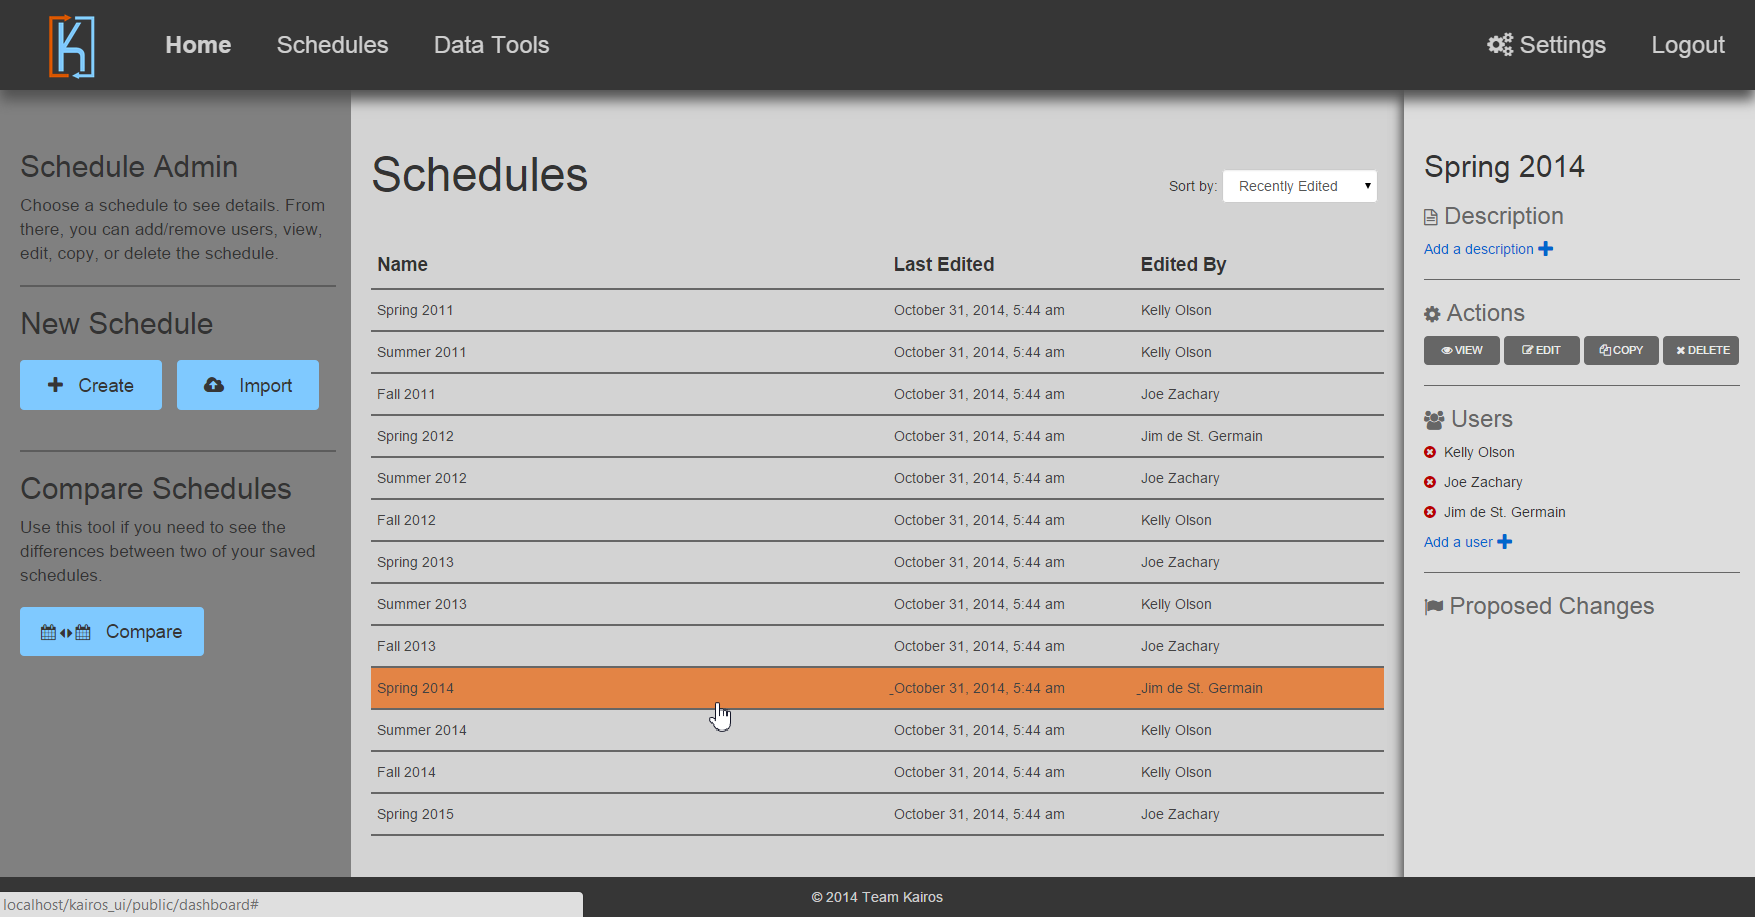
\includegraphics[width=1.0\textwidth]{img/dashboard_02}
    \caption{User schedule selection dashboard}
    \label{fig:dashboard_02}
\end{figure}

\begin{figure}[!ht]
    \centering
    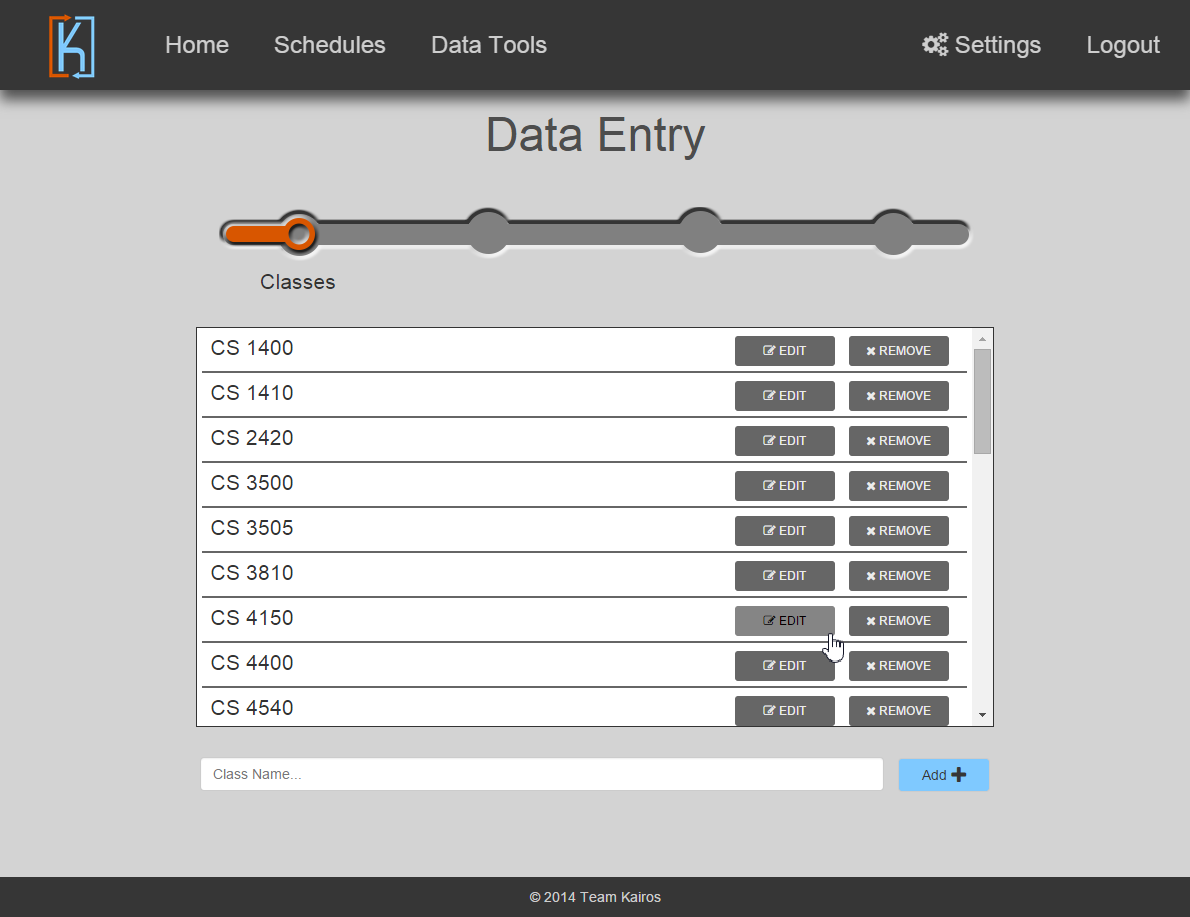
\includegraphics[width=1.0\textwidth]{img/data-entry-classes}
    \caption{User data entry screen for classes}
    \label{fig:data-entry-classes}
\end{figure}

\begin{figure}[!ht]
    \centering
    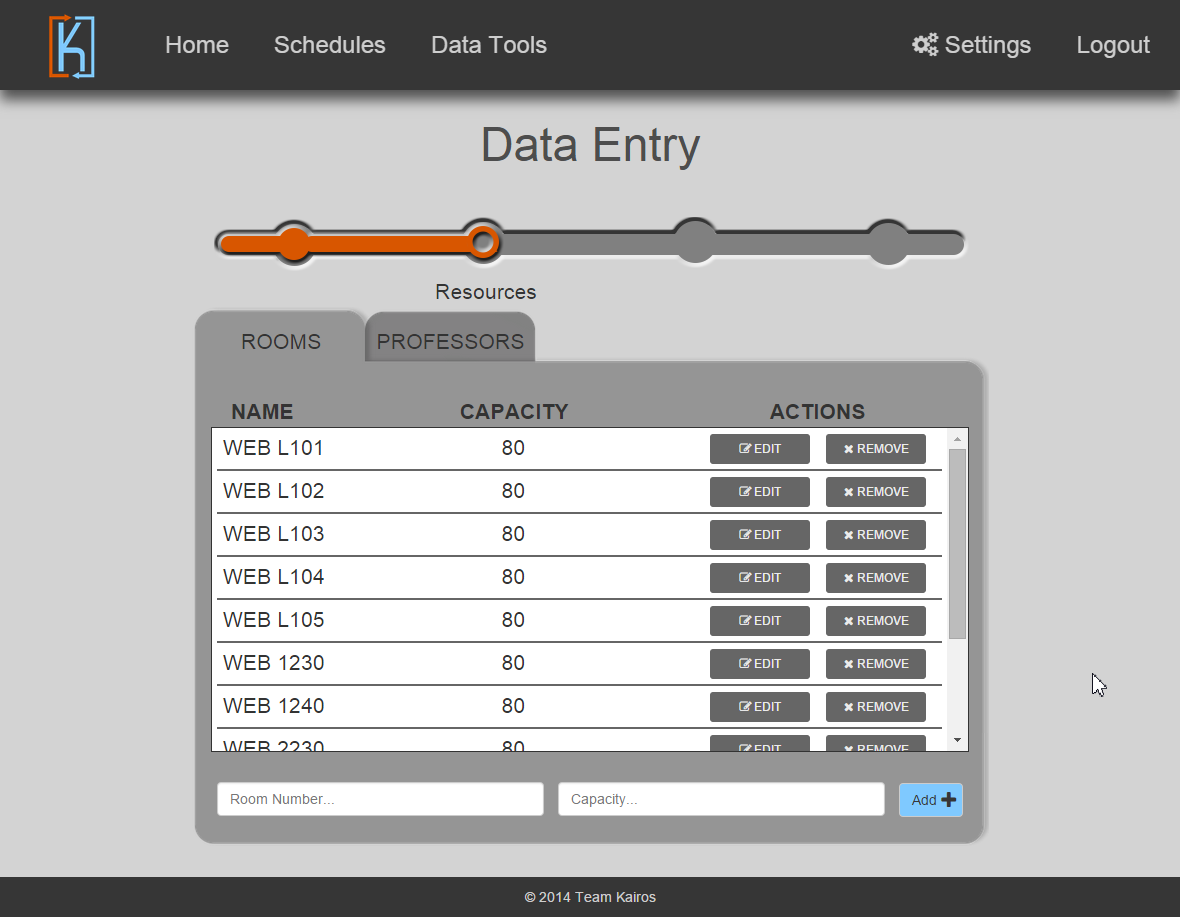
\includegraphics[width=1.0\textwidth]{img/data-entry-rooms}
    \caption{User data entry screen for rooms}
    \label{fig:data-entry-rooms}
\end{figure}

\clearpage{}

\begin{figure}[!ht]
    \centering
    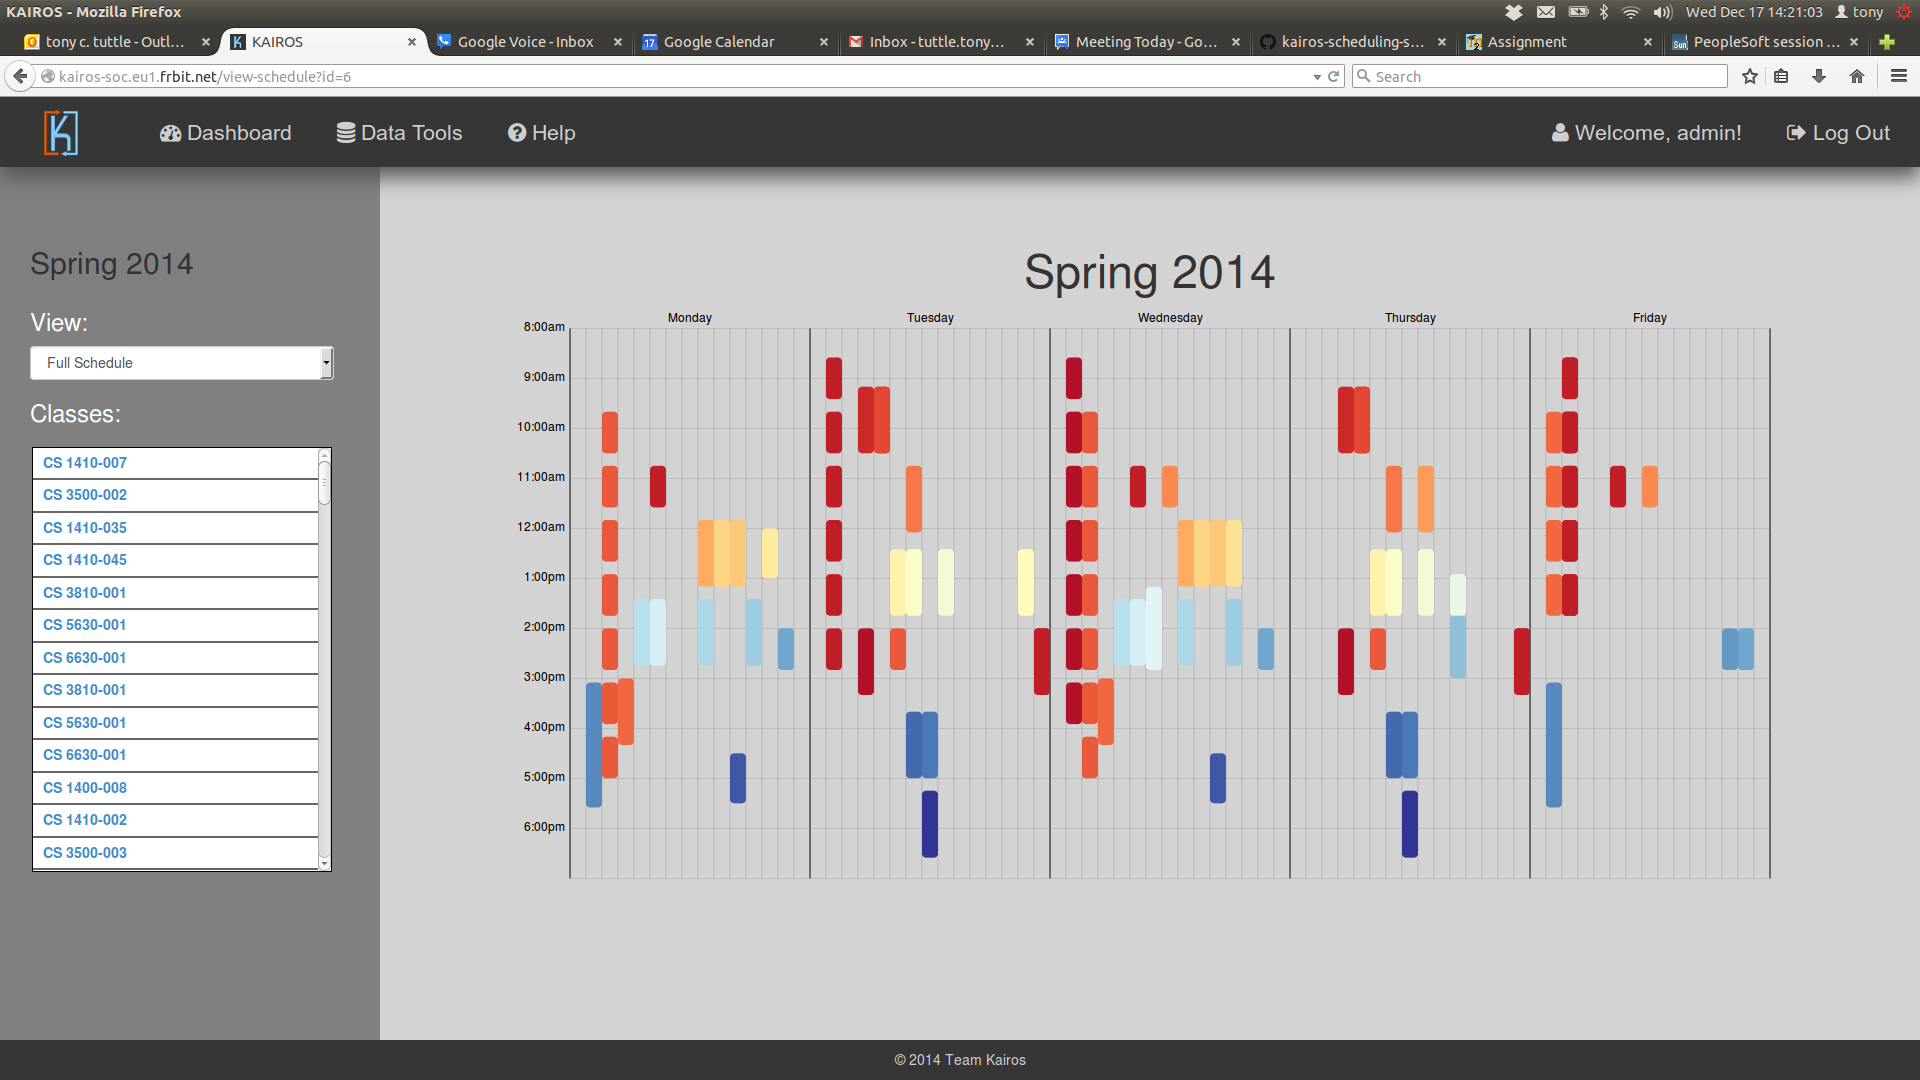
\includegraphics[width=1.0\textwidth]{img/full-sched-view}
    \caption{Visualization of a schedule}
    \label{fig:full-sched-view}
\end{figure}

\begin{figure}[!ht]
    \centering
    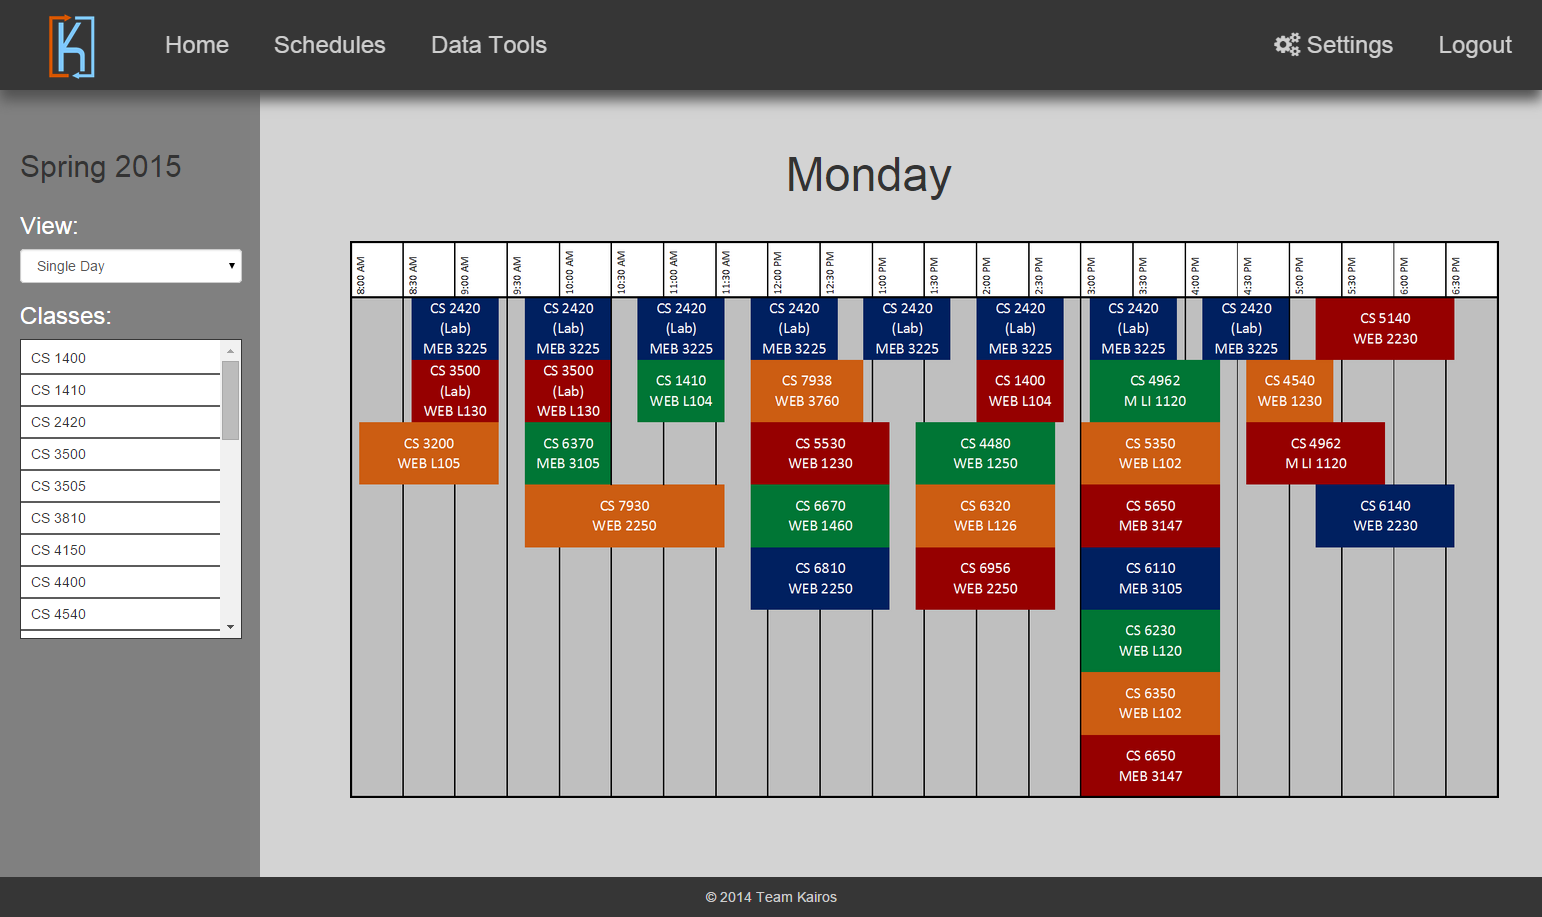
\includegraphics[width=1.0\textwidth]{img/single-day-view}
    \caption{Single day visualization of a schedule}
    \label{fig:single-day-view}
\end{figure}

\begin{figure}[!ht]
    \centering
    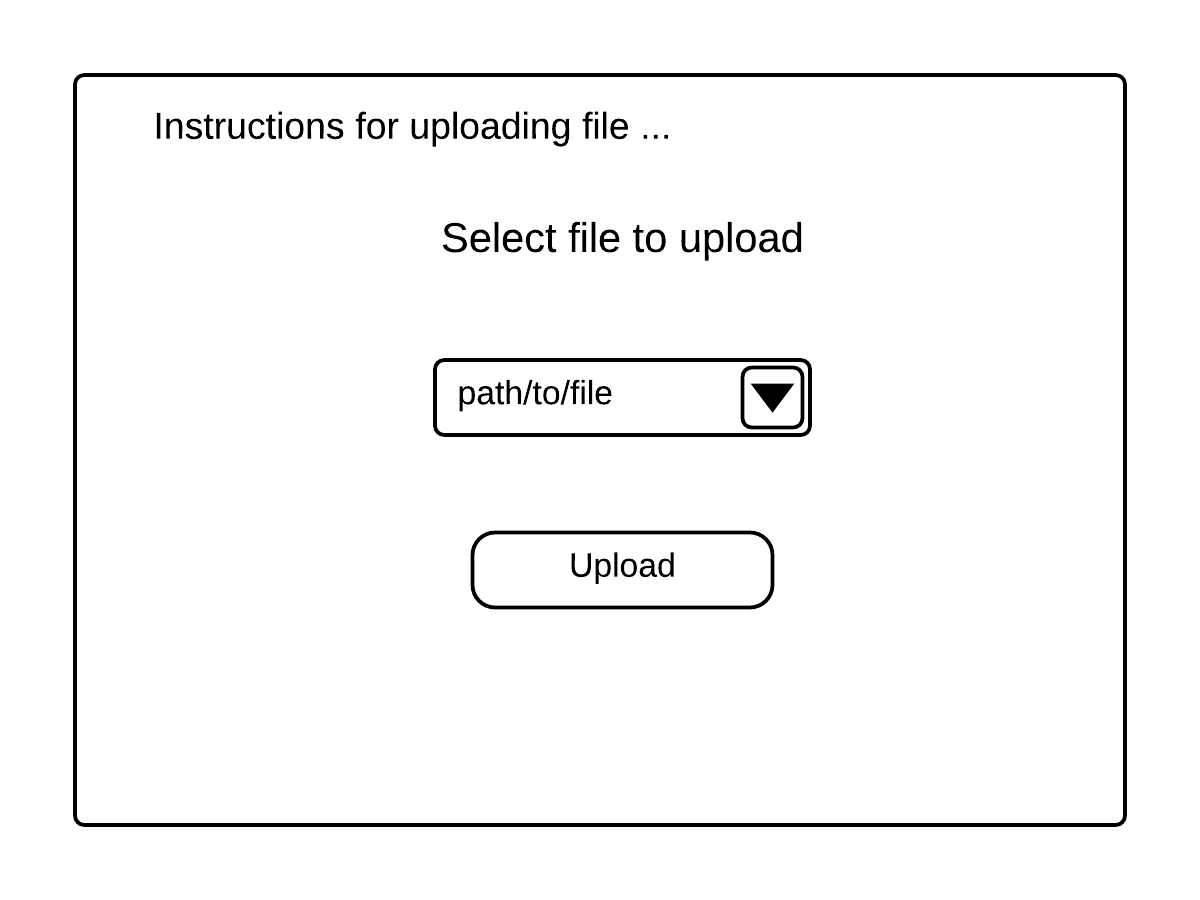
\includegraphics[width=1.0\textwidth]{img/upload_page_wireframe}
    \caption{Wireframe of UI for user to upload a CSV file}
    \label{fig:upload_page_wireframe}
\end{figure}

\begin{figure}[!ht]
    \centering
    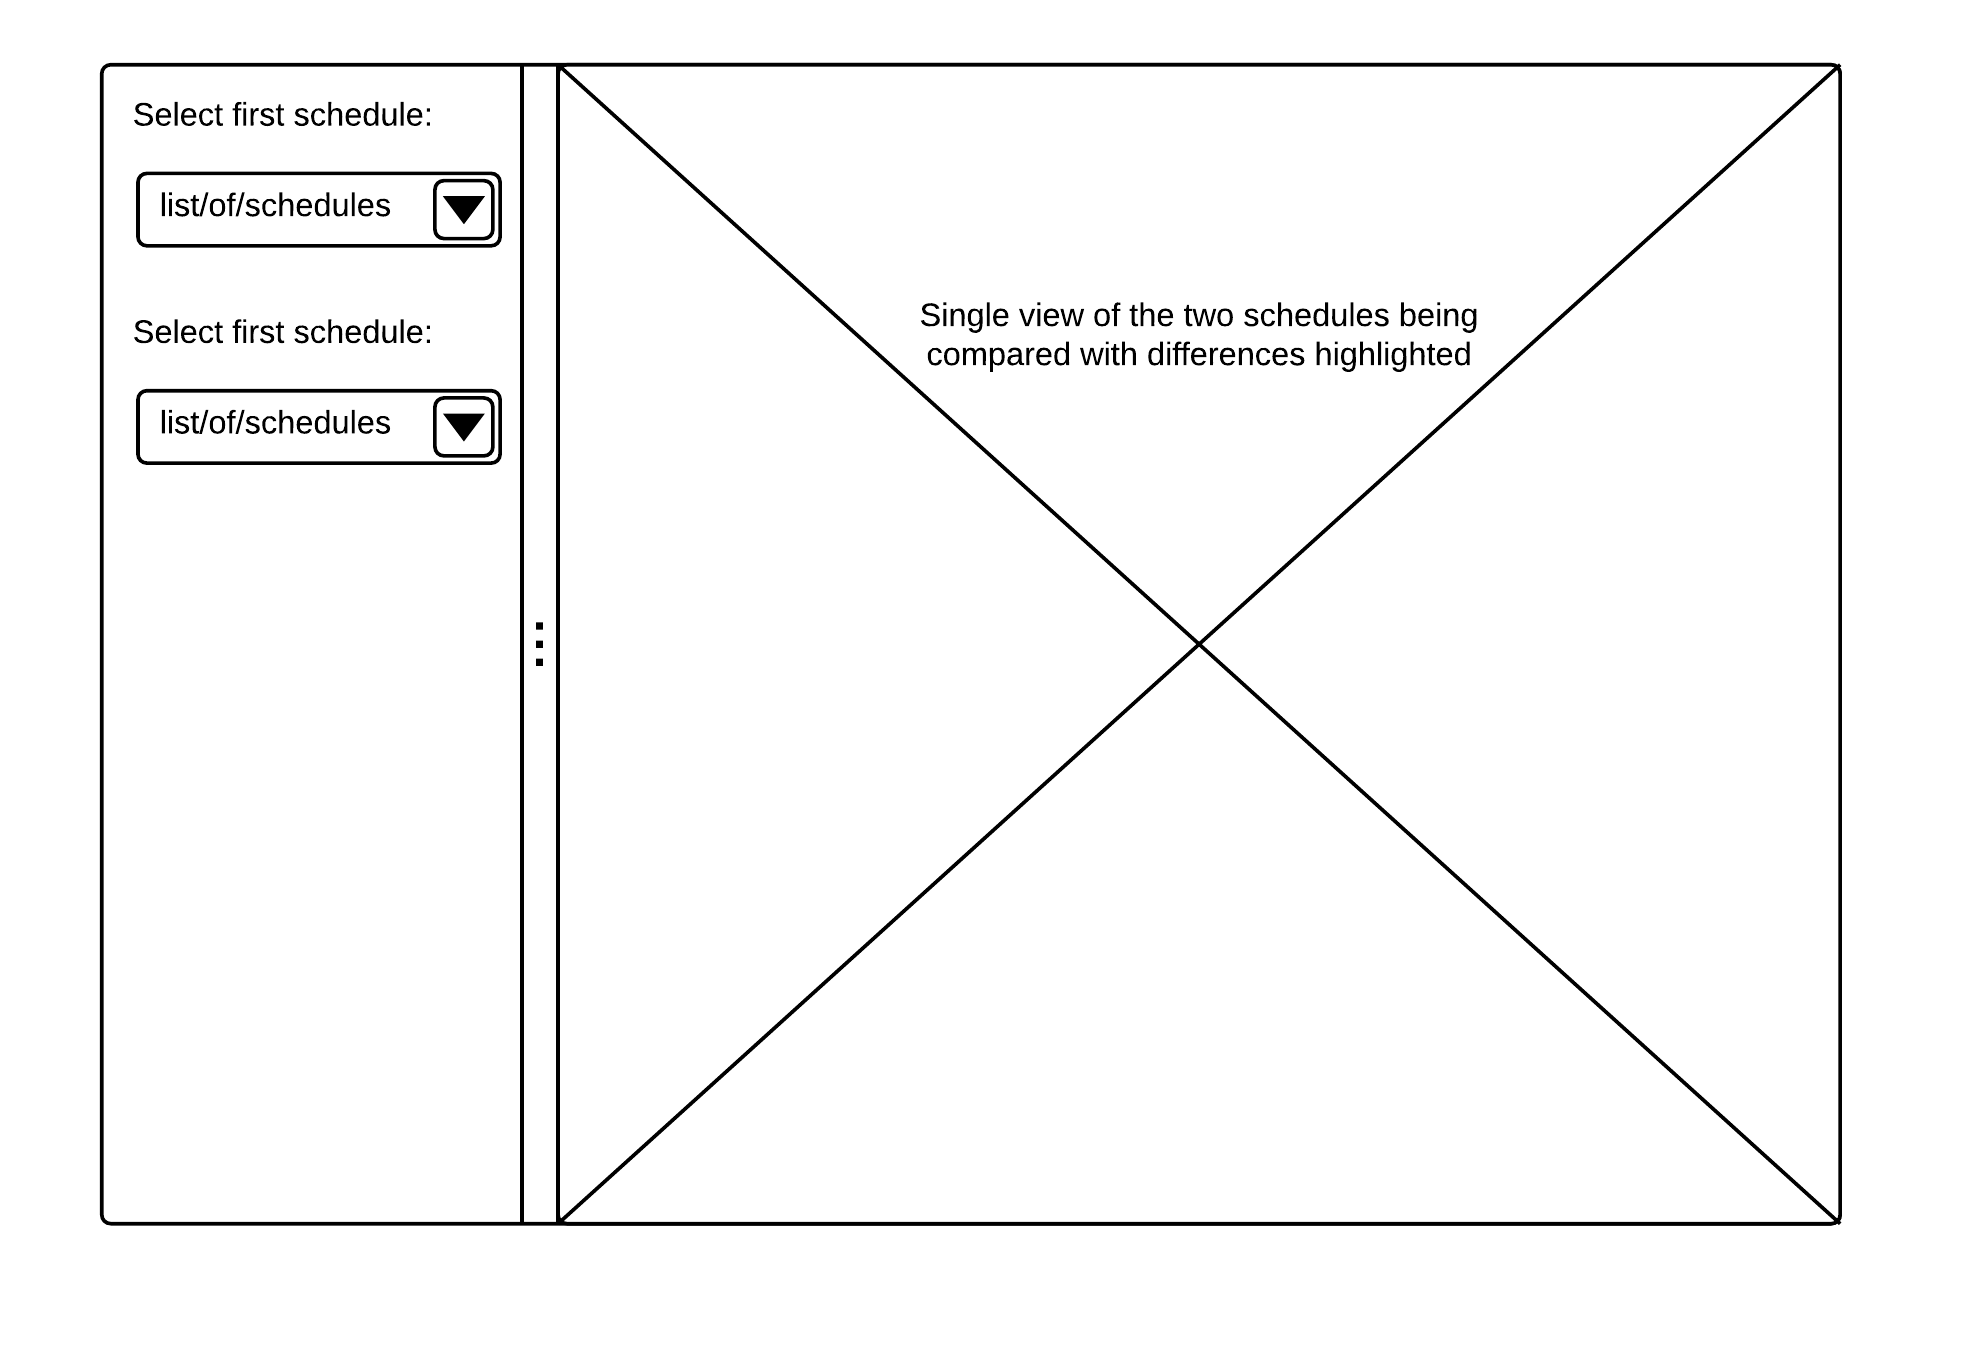
\includegraphics[width=1.0\textwidth]{img/compare_page_wireframe}
    \caption{Wireframe of UI for user to view differences between two schedules}
    \label{fig:compare_page_wireframe}
\end{figure}
\end{appendices}

\end{document}
